
\documentclass{llncs}
%\usepackage{times}
\usepackage{epsfig}
%\usepackage{enumerate}
%\usepackage{paralist}
%\usepackage{amsmath}
%\usepackage{amssymb}
%\usepackage{amscd}
%\usepackage{array}
%\usepackage{tabularx}
\usepackage{xspace}
\usepackage{url}
%\usepackage{float}
\usepackage{multirow}
\usepackage{listings}
%\usepackage{latexsym,pstricks,pst-node,pst-tree,boxedminipage,stmaryrd}
%\usepackage{alltt}
%\usepackage{fancyhdr}
%\usepackage{fullpage}

\usepackage{paralist}
%\markboth{INSPIRED}{INSPIRED}

%\pagestyle{myheadings}

% julien: mes macros
\newcommand{\rarrow}{$\rightarrow$}
\newcommand{\conj}{$\wedge$}
\newcommand{\disjonc}{$\vee$}
\newcommand{\s}{\,}
\newcommand{\btab}{\begin{tt}\begin{tabbing}}
\newcommand{\etab}{\end{tabbing}\end{tt}}
% julien: fin de mes macros
\newcommand{\native}{\texttt{native}\xspace}

\pagestyle{plain}
\title{JACK~---~a tool for validation of security and behaviour of Java
applications\thanks{This work is partially funded by the IST programme
of the European Commission, under the IST-2003-507894
\textsf{Inspired} and IST-2005-015905 \textsf{Mobius} projects.}}

\author{Gilles Barthe\inst{1} \and
        Lilian Burdy\and %\inst{2} \and
        Julien Charles\inst{1} \and
        Benjamin Gr\'egoire\inst{1} \and
        Marieke Huisman\inst{1} \and
        Jean-Louis Lanet\inst{2} \and
        Mariela Pavlova\inst{3}\thanks{Research done while at INRIA Sophia Antipolis.} \and
        Antoine Requet\inst{2}}
\institute{INRIA Sophia Antipolis, France \and 
           gemalto, France \and 
           Ludwig-Maximilians-Universit\"at M\"unchen, Germany}


%\parindent 1cm
%\parskip 0.2cm
%\topmargin 0.2cm
%\oddsidemargin 1cm
%\evensidemargin 0.5cm
%\textwidth 15cm
%\textheight 21cm

%\def\lstlanguagefiles{lstlangjml.sty}
%\lstloadlanguages{Jml}

\newcommand{\benchname}[1]{\texttt{#1}}

\newcommand{\comment}[1]{{\sf #1}}
\newcommand{\alarm}[1]{\marginpar{#1}}

%\newtheorem{definition}{Definition}
%\newtheorem{lemma}{Lemma}
%\newtheorem{theorem}{Theorem}


\def \bsl       {\symbol{92}}
\def \unsc      {\symbol{95}}

\newcommand{\todo}[1]{ \textbf{#1}}
\newcommand{\fig}[1]{ Fig.}
\newcommand{\jmlKey}[1]{\texttt{#1}}% wrapping jml keywords
\newcommand{\java}[1]{\texttt{#1}}
\newcommand{\stack}[1]{\texttt{st(#1)}}% element on top stack 
\newcommand{\counter}{\texttt{ct}}

\newcommand{\true}{\texttt{true}}
\newcommand{\false}{\texttt{false}}

\newcommand{\wpi}{\textit{wp}}

\newcommand{\instr}[1]{\texttt{#1}}

\newcommand{\substitution}[2]{[\tt{#1} \leftarrow \tt{#2}]}
% thegrammar for the bytecode specification language
\newcommand{\ClassSpec}{\rm{ClassSpec}}
\newcommand{\MethodSpec}{\rm{MethodSpec}}
\newcommand{\SpecCase}{\textrm{SpecCase}}
\newcommand{\jmlStmt}[1]{\textrm{#1}}
\newcommand{\interMethodSpec}{\rm{InterMethodSpec}}
\newcommand{\loopSpec}{\rm{loopSpec}}
%\newcommand{\assert}{\rm{assertSpec}}

\newcommand{\ArithExpr}{\texttt{Arithmetic\_Expr}}
\newcommand{\expression}{\mathcal{E} }

\newcommand{\integer}{\texttt{int} }
\newcommand{\register}[1]{\texttt{lv[#1]} }
\newcommand{\reference}{\texttt{ref} }
\newcommand{\intLiteral}{\texttt{int\_literal} }
\newcommand{\Mynull}{\texttt{null}}
\newcommand{\this}{\texttt{this}}
\newcommand{\fieldAccess}[1]{\texttt{field\_cp\_index(}#1 \texttt{)}}
\newcommand{\arrayAccess}[2]{#1[#2] }

\newcommand{\result}{\jmlKey{$\backslash$result}}
\newcommand{\oldp}[1]{\jmlKey{$\backslash$old(}#1\jmlKey{)}}
\newcommand{\typeof}[1]{\jmlKey{$\backslash$typeof(}#1 \jmlKey{)}}
\newcommand{\EXC}{\texttt{EXC}}

\newcommand{\excPost}{\psi^{exc}}

\newcommand{\Myspace}{\phantom{aa}}
\newcommand{\predicate}{ \mathcal{P}} 
\newcommand{\Myfalse}{\textit{false}}
\newcommand{\Mytrue}{ \textit{true} }
\newtheorem{defn}{Definition} 



% abstractCtrlFlow.tex
\newcommand{\execRel}{\rightarrow} % the execution relation
\newcommand{\blockm}[1]{ \tt{b^{#1}} }
\newcommand{\blockSeq}[1]{ \tt{b_{seq}^{#1}} }
%\newcommand{\pathm}[2]{\blockm{#1} \execRel^{*} \blockm{#2} }

\newcommand{\blockPost}[1]{ \it{post(}\tt{b_{seq}^{#1}}\it{)}}

\newcommand{\invariant}{\textit{I}}

\newcommand{\srcVar}[1]{\texttt{#1} }

\newcommand{\method}{\texttt{m}}

% recuperé dans le prelude du code généré par l'Atelier B.
% Doit permettre d'écrire à peu-près correctement <+
\def\famletter#1{\ifcase #1 0\or 1\or 2\or 3\or 4\or 5\or 6\or 7\or
    8\or 9\or A\or B\or C\or D\or E\or F\fi}
\font\msx=msam10
\newfam\msxfam \textfont\msxfam=\msx
\edef\fx{\famletter\msxfam}
\mathchardef    \dres       "2\fx43
\def    \lover      {\mathbin{{\dres} \llap{$-\!\!\!\!-\!$}}}

\def\keywords{\noindent\bf Keywords: \vspace{0pt}
\it\normalsize\normalsize}
\def\endkeywords{\par}

\def\acknowledgement{\vspace{4pt} \noindent{\bf Acknowledgements} \\ \vspace{1pt}
\normalsize\normalsize}
\def\endkeywords{\par}

\newcommand{\JACK}{\texttt{JACK}}
\newcommand{\ESC}{\texttt{ESC/Java}}
\newcommand{\LOOP}{\texttt{LOOP}}


\date{}
\newcommand{\bbb}{\mathbb{B}}
% moved here from carmel.tex
\newcommand{\spp}{\hspace{1.5cm}}


\newcommand{\semb}{\llbracket}
\newcommand{\seme}{\rrbracket}
\newcommand{\sem}[1]{ \semb #1 \seme}
\newcommand{\ia}[1]{ \semb #1 \seme}
\newcommand{\fia}[1]{ \mathcal{F}\semb #1 \seme}
\newcommand{\ria}[1]{ \mathcal{R}\semb #1 \seme}

\newcommand{\Coq}{{\sf Coq}}
\newcommand{\ocaml}{\textsc{ocaml}}

\newcommand{\memvar}{\text{Mem}}

\newcommand{\AbVal}{\widehat{\text{Val}}}
\newcommand{\Val}{{\text{Val}}}
%\newcommand{\Stack}{{\text{Stack}}}
\newcommand{\AbStack}{{\widehat{\text{Stack}}}}
\newcommand{\SafeCallStack}{{\text{SafeCallStack}}}
\newcommand{\OneCall}{{\text{OneCall}}}
\newcommand{\Var}{{\text{Var}}}
\newcommand{\LocalVar}{{\text{LocalVar}}}
\newcommand{\AbLocalVar}{{\widehat{\text{LocalVar}}}}
\newcommand{\State}{{\text{State}}}
\newcommand{\Trace}{{\text{Trace}}}
\newcommand{\AbState}{{\widehat{\text{State}}}}
\newcommand{\progCount}{{\text{progCount}}}
\newcommand{\fieldName}{{\text{fieldName}}}
\newcommand{\methodName}{{\mathrm{methodName}}}
\newcommand{\MM}{{\methodName}}
\newcommand{\PP}{{\progCount}}
\newcommand{\className}{{\text{className}}}
\newcommand{\varName}{{\text{varName}}}
\newcommand{\Adress}{{\text{Adress}}}
\newcommand{\Instruction}{{\text{Instruction}}}
\newcommand{\InstAt}{{\text{InstAt}}}
\newcommand{\Constraint}{{\text{Constraint}}}
\newcommand{\St}{\widehat{\text{St}}}

\newcommand{\config}[1]{{\langle\!\langle #1 \rangle\!\rangle}}
\newcommand{\fram}[1]{{\left\langle #1 \right\rangle}}
\newcommand{\num}{{\text{num}}}
\newcommand{\reff}{{\text{ref}}}
\newcommand{\nul}{{\text{null}}}
\newcommand{\some}{{\text{some}}}
\newcommand{\nameClass}{{\text{nameClass}}}
\newcommand{\class}{{\text{class}}}
\newcommand{\newObject}{{\text{newObject}}}
\newcommand{\newArray}{{\text{newArray}}}
\newcommand{\lengthArray}{{\text{lengthArray}}}
\newcommand{\fieldValue}{{\text{fieldValue}}}
\newcommand{\Value}{{\text{Value}}}
\newcommand{\classes}{{\text{classes}}}
\newcommand{\RefValue}{{\text{RefValue}}}
\newcommand{\Location}{{\text{Location}}}
\newcommand{\methodLookup}{{\text{methodLookup}}}
\newcommand{\nbArgument}{{\text{nbArgument}}}
\newcommand{\nameMethod}{{\text{nameMethod}}}

\newcommand{\ClassName}{{{\text{ClassName}}}}
\newcommand{\FieldName}{{{\text{FieldName}}}}
\newcommand{\default}{{{\text{default}}}}
\newcommand{\END}{{{\text{END}}}}
\newcommand{\AbHeap}{{\widehat{\text{Heap}}}}

\newcommand{\Sinit}{{\mathcal{S}_{\mathit{init}}}}

\newcommand{\instructionAt}{{\text{instructionAt}}}


%\newcommand{\abs}{\mbox{${\cal S}\!\mathit{t}$}}
\newcommand{\abs}{\mbox{$\Sigma$}}
\newcommand{\addr}{\mbox{\em addr}}
\newcommand{\pc}{\mathit{pc}}
\newcommand{\stf}{{\mathit{sf}}}
\newcommand{\cl}{{\mathit{cl}}}

\newcommand{\analyze}{\text{\tt analyse}}
\newcommand{\Analyze}{\ensuremath{\mathit{Unbounded}(P)}}
\newcommand{\Program}{\text{Program}}

\newenvironment{constraint}{%
\noindent
\hspace{.3mm}$
\begin{array}[t]{l}}{%
\end{array}$\\[0.2cm]
}

\newenvironment{contraint}{%
\noindent
\hspace{1cm}$
\begin{array}[t]{l}}{%
\end{array}$\\[0.5cm]
}




\newcommand{\AbPop}{\widehat{\text{pop}}}
\newcommand{\AbPush}{\widehat{\text{push}}}
\newcommand{\AbTop}{\widehat{\text{top}}}
\newcommand{\AbBinop}{\widehat{\text{binop}}}
\newcommand{\AbApply}{\widehat{\text{apply}}}
\newcommand{\AbSubst}{\widehat{\text{subst}}}
\newcommand{\Num}{{{\text{Num}}}}
\newcommand{\AbNum}{{\widehat{\text{Num}}}}
\newcommand{\AbRef}{{\widehat{\text{Ref}}}}
\newcommand{\AbObject}{{\widehat{\text{Object}}}}
%\newcommand{\AbHeap}{{\widehat{\text{Heap}}}}
\newcommand{\Flow}{\text{\tt Flow}}

\newenvironment{myalltt}{\vspace*{-3pt}\begin{alltt}}{\end{alltt}\vspace*{-3pt}}

%%
%% Added by Gerardo (28/09/2004)
%%

\newcommand{\Rule}[2]
{
\frac{#1}
{
\begin{array}{l}
#2
\end{array}
}
}

\newcommand\Loop{\ensuremath{\mathit{Loop}}}
\newcommand\Pred{\ensuremath{\mathit{Pred}}}
\newcommand\BC{\ensuremath{\mathit{BC}}}
\newcommand\MutRec{\ensuremath{\mathit{MutRecR}}}
\newcommand\Rec{\ensuremath{\mathit{Rec}}}
\newcommand\Anc{\ensuremath{\mathit{Anc}}}
\newcommand\LoopCall{\ensuremath{\mathit{LoopCall}}}
\newcommand\Call{\ensuremath{\mathit{Call}}}
\newcommand\Q{\ensuremath{\mathit{Q}}}
\newcommand\tr{\ensuremath{\mathit{tr}}}

\newcommand\End{\ensuremath{\mathtt{end}}}
\newcommand\nop{\ensuremath{\mathtt{nop}}}
\newcommand\push{\ensuremath{\mathtt{push}}}
\newcommand\pop{\ensuremath{\mathtt{pop}}}
\newcommand\dup{\ensuremath{\mathtt{dup}}}
\newcommand\swap{\ensuremath{\mathtt{swap}}}
\newcommand\numop{\ensuremath{\mathtt{numop}}}
\newcommand\load{\ensuremath{\mathtt{load}}}
\newcommand\store{\ensuremath{\mathtt{store}}}
\newcommand\inc{\ensuremath{\mathtt{inc}}}
\newcommand\add{\ensuremath{\mathtt{add}}}
\newcommand\sub{\ensuremath{\mathtt{sub}}}
\newcommand\goto{\ensuremath{\mathtt{goto}}}
\newcommand\If{\ensuremath{\mathtt{if}}}
\newcommand\looksw{\ensuremath{\mathtt{lookupswitch}}}
\newcommand\tabsw{\ensuremath{\mathtt{tableswitch}}}
\newcommand\newarray{\ensuremath{\mathtt{newarray}}}
%\newcommand\default{\ensuremath{\mathtt{default}}}
\newcommand\new{\ensuremath{\mathtt{new}}}
\newcommand\checkc{\ensuremath{\mathtt{checkcast}}}
\newcommand\getst{\ensuremath{\mathtt{getstatic}}}
\newcommand\putst{\ensuremath{\mathtt{putstatic}}}
\newcommand\instof{\ensuremath{\mathtt{instanceof}}}
\newcommand\getfd{\ensuremath{\mathtt{getfield}}}
\newcommand\getfdt{\ensuremath{\mathtt{getfield this}}}
\newcommand\putfd{\ensuremath{\mathtt{putfield}}}
\newcommand\invdef{\ensuremath{\mathtt{invokedefinite}}}
\newcommand\invvir{\ensuremath{\mathtt{invokevirtual}}}
\newcommand\invint{\ensuremath{\mathtt{invokeinterface}}}
\newcommand\return{\ensuremath{\mathtt{return}}}
\newcommand\arrlh{\ensuremath{\mathtt{arraylength}}}
\newcommand\arrld{\ensuremath{\mathtt{arrayload}}}
\newcommand\arrst{\ensuremath{\mathtt{arraystore}}}
\newcommand\throw{\ensuremath{\mathtt{throw}}}
\newcommand\jsr{\ensuremath{\mathtt{jsr}}}
\newcommand\ret{\ensuremath{\mathtt{ret}}}
\newcommand\thiss{\ensuremath{\mathtt{this}}}
%\newcommand\instr{\ensuremath{\mathtt{instr}}}
\newcommand\const{\ensuremath{\mathtt{const}}}
\newcommand\Array{\ensuremath{\mathsf{array}}}
\newcommand\Int{\ensuremath{\mathsf{int}}}
\newcommand\byte{\ensuremath{\mathsf{byte}}}
\newcommand\short{\ensuremath{\mathsf{short}}}
\newcommand\bool{\ensuremath{\mathsf{bool}}}
\newcommand\Ctxt{\ensuremath{\mathsf{Ctxt}}}

\newcommand\warn{\ensuremath{<!>}}
\newcommand\trace{\overline{s}}
\newcommand\defi{\stackrel{\mathrm{def}}{=}}
\newcommand\lub{\sqcup}

\newcommand\Size{\ensuremath{\mathit{Size}}}
\newcommand\Pre{\ensuremath{\mathrm{Pre}}}
\newcommand\Post{\ensuremath{\mathrm{Post}}}
\newcommand\old{\ensuremath{\backslash\mathrm{old}}}

%%%%%%%%%%%%%%%%%%%%%%%%%%%%%%%%%%%%%%%%%%%%%%%%%%%%%%%
%%
%% Mariela's definitions
%%
%%%%%%%%%%%%%%%%%%%%%%%%%%%%%%%%%%%%%%%%%%%%%%%%%%%%%%%


%\newcommand{\pathm}[2]{\blockm{#1} $\ll^{*}$ \blockm{#2} }



%%%%%%%%%Specification commands
\newcommand{\annotation}{BML}
\newcommand{\Apredicate}{\textit{P}}


\newcommand{\requires}{\texttt{requires}}
\newcommand{\ensures}{\texttt{ensures}}
\newcommand{\exsures}[1]{\texttt{exsures(#1)}}
\newcommand{\assert}{\texttt{assert}}

\newcommand{\variant}{\texttt{variant}}

\newcommand{\declare}{\texttt{declare}}
\newcommand{\ghost}{\texttt{Model}}
\newcommand{\ghostSet}{\texttt{set}}
\newcommand{\modifies}{\texttt{modifies}}
\newcommand{\ensemble}[2]{#1 .. #2}
\newcommand{\maxIter}[1]{ iter^#1 }
\newcommand{\progLoop}[1]{\textit{#1}}
\newcommand{\memConsAt}[1]{\Mem^l}

\newcommand{\atState}[2]{#1^{#2} }

%\newcommand{\Mem}{\texttt{MemUsed}}
\newcommand{\Mem}{\texttt{Mem}}
%\newcommand{\old}{\texttt{old}}
\newcommand\Max{\ensuremath{\texttt{Max}}}
\newcommand{\allocated}[1]{allocPath(#1)}
\newcommand{\srcCode}[1]{\texttt{#1}}
\newcommand{\local}[1]{\texttt{localVar}(#1)}



%%%%%%%%%%%% allocation function
\newcommand{\visited}{\texttt{visited}}



%\newcommand{\instrAt}[1]{i_{#1}}
%\newcommand{\instanceOfAlloc}[1]{instanceOfAllocates( #1 )}

\newcommand{\allocInstance}[1]{\texttt{allocInst(#1)}}
\newcommand{\allocLoop}[1]{\texttt{loopCon(#1)}} % function that returns directly the allocations done by a loop : multiplied by the max iterations it can do
\newcommand{\allocMethod}[1]{\texttt{mthdCon(#1)}} % returns the allocations done in a method
\newcommand{\allocLoopWithEnd}[2]{alloc\_loop\_path(#1 , #2)} % returns the allocations done in a loop for a particular path that starts at the start instruction of a loop and that % ends with an insstruction that leads back to the start instructions

\newcommand{\allocIns}[1]{alloc\_instr(#1)} % function that returns that the allocation by the argument

\newcommand{\numLoop}[1]{\textit{numberLoop}(#1)}
\newcommand{\loopEndsSet}[1]{loopEndSet(#1)}
\newcommand{\loopSet}[1]{loopSet(#1)}
\newcommand{\loopEntry}[1]{entry(#1)} % predicate that says that the instruction is an entry to a loop

\newcommand{\backedge}[2]{backedge(#1,#2)} % the start of the backedge  and the end of the backedge


%\newcommand{\wpi}[3]{ \rm{wp}( \srcCode{#1}, #2, #3) } % wp for instructions
\newcommand{\wpExe}[1]{ \rm{wp}(#1) } % wp for blocks
\newcommand{\normalPost}{\psi^{n}}


%\newcommand{\stack}[1]{St(#1)}
\newcommand{\topStack}{c}
\newcommand{\javaNull}{null}
\newcommand{\Ref}[1]{ref_{#1} }
\newcommand{\NULL}{\texttt{null}}



\newcommand{\prevIns}[1]{prev(#1 )}
\newcommand{\nextIns}[1]{next(#1 )}
\newcommand{\targetIns}[1]{target(#1)}



%%%%%%%%%%%%%%%%%%%%%%%%%%%%%%%%%%%%%%%%%%%%%%%%%%%%%


          % input user-defined commands

\begin{document}
\maketitle      
\begin{abstract}
We describe the main features of JACK (Java Applet Correctness Kit), a
tool for the validation of Java applications, annotated with JML
specifications. JACK has been especially designed to improve the
quality of trusted personal device applications. JACK is fully
integrated with the IDE Eclipse, and provides an easily accessible
user interface. In particular, it allows to inspect the generated
proof obligations in a Java syntax, and to trace them back to the
source code that gave rise to them. Further, JACK provides support for
annotation generation, and for interactive verification. The whole
platform works both for source code and for bytecode, which makes it
particularly suitable for a proof carrying code scenario.
\end{abstract}
Java is a language commonly used on small device, with specific flavour
of it being used on heterogenous devices like cellphones or JavaCards. 
Thus taking into account their specific caracteristic each implementations
is important for verification.
Especially if specific system components change the overall behaviour of JVMs. 
Verification of system components is scattered through
litterature: there has been verifications of bytecode verifiers, as
well as access contoller. As far as our knowledge goes
though~\cite{HartelMoreau01}, the Security Manager of the JVM 
has not been verified and its semantic is not taken into
account when usually doing static verification of Java programs.


The main goal of this paper is to verify an implementation of a
Security Manager, and also to give a framework to more generally verify
programs taking into account the semantic differences that different
component of the JVM can bring to executions of program inside 
a JVM.

\vspace{-0.4cm}
\subsection{The Security Manager}
The Security Manager applies the security policies on two
levels. First on the library level: each time a writing or reading
operation is called for instance a call to the Security Manager is
made and if the caller has not respected a given security policy, a
{\tt SecurityException} is thrown.
Second on the JVM level: each time a class is
loaded, it checks on a meta level with the use of the ClassLoader
(which for this paper will be considered as a part of the JVM) if the
currently inspected class has the right to access a specified type
from an outside package.  
The latter is hard to take into account for a program verification, 
because it changes the behavior of type resolution which is part
of the language semantic.  A practical way to
model these changes would be to consider the Security Manager as an
Aspect which would weave at the cutting points representing type
resolution.
\vspace{-0.4cm}
\begin{figure}
\bcode
pa\=ckage a;\\
public class Main \{\+\\
  st\=atic \{\+\\
    Sy\=stem.setSecurityManager(new SecurityManager() \{\+\\
      pu\=blic void checkPackageAccess(String target) \{\+\\
        if\=(target.equals("b"))\\
          \>throw new SecurityException("That is true");\\
      \}\});\-\-\\
  \}\\
 \\
  public static void main(String[] args) \{\+\\
    System.out.println("Nextline will throw an exception");\\
    b.A a = new b.A();\-\\
  \}\-\\
\}
\ecode
The output of the program:
\bcode
Next line will throw an exception\\
Excepti\=on in thread "main" java.lang.SecurityException: That is true\+\\
	at a.b.Main\$1.checkPackageAccess(Main.java:9)\\
	\dots
\ecode
\caption{An invasive Security Manager}
\end{figure}

\vspace{-1cm}
\subsection{Modeling with AspectJ}
Aspect Oriented Programming (AOP) is a paradigm that offers
modularity though it is ortogonal to the usual Object Oriented
Programming paradigm. AOP enables to weave code directly into a
program,  changing the behaviour of given language constructs. Two new
notions have been introduced through AOP:
\begin{itemize}
\item the concept of cutting points, points in the program where code
can be inserted, and
\item advices, code to be inserted at a specified cutting point.
\end{itemize}
AspectJ is one of the most popular of the AOP languages. It is Java-based, 
so it is a natural choice for modelling the Security Manager through aspects.

Implementing the Security Manager as an invasive Aspect is easy.  As
we have seen in the above example, a minimal Security Manager could
change the behaviour of the JVM at the type access step. The
difficulty here would be that the type is checked only on the first
call, for this purpose a field has to be introduced, as shown in
Figure \ref{base_implem}.
%
\vspace{-0.4cm}
\begin{figure}
\bcode
pu\=blic aspect SecurityManager \{\+\\

Set$<$String$>$ s = new HashSet$<$String$>$();\\
po\=intcut anyPublicMethod(Object o) : \=target(o) \&\& !within(SecurityManager)\+ \\
           \>\&\& call( public *(*))\-\\
before(Object o) : anyPublicMethod(o) \{\+\\
    String pkg = o.getClass().getPackage().toString();\\
    if\=(!s.contains(pkg)) \{\+\\     
       s.add(pkg);\\
       if\=(pkg.equals("b"))\\
           \>throw new SecurityException("That is true");\\\-\\ 
    \}\-\\
\}\-\\
\}
\ecode
\caption{An Aspect implementation of the invasive SecurityManager}
\label{base_implem}
\end{figure}
\vspace{-1cm}
\subsection{Verification framework}
\label{framework}
The verification framework we will use to handle the Security Manager concerns 
is an adaptation of static verification techniques based on weakest
precondition calculus. It is inspired by Java extended static verification
tools that use guarded commands language like ESC/Java2~\cite{CokK04} and
the Mobius PVE~\cite{MobiusPVE07}.


The verification process is made of several steps:
First the program and the aspects have to be fully specified:
\begin{enumerate}
\item the program and its aspects are annotated using an aspect specific
behavioural specification language, Pipa,
\item the behavioural specifications are desugared
\item the aspects are abstracted to models
\end{enumerate}
Then the proper compilation of aspects is done:
\begin{enumerate}
\item the program is compiled to bytecode with its specifications
\item the program is transformed into guarded commands
\item the model methods representing advices are weaved into the program
\end{enumerate}
Finally a weakest precondition calculus is made on the transformed
program, and verification conditions are generated in order to be
solved automatically or interactively.

\vspace{-0.4cm}
\subsection{Related Work}
\label{related}
In this paper we focus on a verification framework adapted for the
verification of AspectJ programs annotated with Pipa.  The pointcut
semantic of AspectJ has been properly
defined~\cite{DBLP:conf/popl/AvgustinovHOMSTV07} as well as the advice
weaving semantic~\cite{weaving04} though only parts have been
formalized~\cite{weaving06}.  Pipa is an annotation language which was
inspired by Clifton and Leavens' work~\cite{clifton02observers}. There
are some extensions to it like pointcuts
annotations~\cite{pointcuts07}, or Moxa \cite{moxa05}.  Our framework
relies on verification based on an intermediate language, like what is
done in ESC/Java2~\cite{FlanaganLLNSS02}, Boogie~\cite{BarnettCDJL05},
or Krakatoa~\cite{MarcheP-MU04}. The work is made to be adapted on a
BoogiePL-like guarded command which is coupled with a
VCGen~\cite{BarnettL05,FlanaganS01}.

\paragraph{Modular verification of Aspects}
Verification in Aspect Oriented Programming language is often linked
to a modular approach.  It is orthogonal to the aim of this paperh: we
tailor verification of aspects which were not specially wanted by the
user, and are most-likely imposed by the environment.  Clifton and
Leavens~\cite{clifton02observers,clifton02spectators,cliftonPhd}
propose a programming discipline to define and specify aspects, using
an extension of JML as specification language.  They define two kind
of aspects, the \emph{spectators} and \emph{assistants} and propose to
explicitly allows the weaving of these aspects. This approach allows
efficient modular reasonning and easy implementations because they
show a way of weaving specifications using a control-flow graph
analysis. In their 2004 work~\cite{shriram04} Krishnamurthi {\it et
al} present a model-checking framework for verification of programs
containing aspects. It is quite different from our work as it presents
a generic framework for aspects. In an unpublished paper~\cite{cesar},
Kunz presents a Hoare logic for modular verification of aspects. The
paper is quite formal, but he does not add special annotations for method
specifications as Clifton and Leavens. For this reason his approach remains 
less modular than Clifton's, but more expressive.




% Shmuel Katz et al. \cite{Katz06,GoldmanK06} propose
% a classification of aspects as \emph{spectative}, \emph{regulative} or
% \emph{invasive}, to simplify program verification by focusing on the









\vspace{-0.4cm}
\subsubsection{Outline:}
First, in Section \ref{specs} we will show how the program has to be
 properly annotated. Then in Section \ref{transf} we will
transform the program to ease its verification: the aspects will be turned
into model methods and the main program code into guarded commands.
In section \ref{verif} we will explain how to verify the transformed program
and finally give a conclusion in Section \ref{conclusion}.

        
\chapter{Java Validation}
\section{Java}
\section{JML}
JML~\cite{Leavens-Baker-Ruby99b,Leavens-Baker-Ruby03}, the
``Java Modeling Language'', is a behavioral interface
specification language for Java; that is, it specifies both the behavior
and the syntactic interface of Java code.  The syntactic interface of
a Java class or interface consists of its method signatures,
the names and types of its fields, etc.
This is what is commonly meant by an application programming
interface (API).
The behavior of such an API can be precisely documented in JML annotations;
these describe the intended way that programmers should
use the API.  In terms of behavior, JML can detail, for example, the
preconditions and postconditions for methods as well as class
invariants.

An important goal for the design of JML is that it should be easily
understandable by Java programmers. This is achieved by staying as
close as possible to Java syntax and semantics.  Another important
design goal is that JML {\em not} impose any particular design method
on users; instead, JML should be able to document Java programs
designed in any manner \cite{Leavens-Baker-Ruby03}.

\label{notation}

JML uses Java's expression syntax in assertions,
thus JML's notation is easy for programmers to learn.  
Because JML supports quantifiers such as
\verb_\forall_ and \verb_\exists_, and because JML allows ``model''
(i.e., specification-only) fields and methods, specifications can
easily be made precise and complete.

JML assertions are written as special
annotation comments in Java code,
so that they are ignored by Java compilers but can be used
by tools that support JML\@.  Within annotation comments JML extends the
Java syntax with several keywords.  It also extends Java's expression syntax with several
operators.

The central ingredients of a JML specification are preconditions
(given in {\tt requires} clauses), postconditions (given in {\tt
  ensures} clauses), and (class and interface) invariants.  These are
all expressed as boolean expressions in JML's extension to Java's
expression syntax.

In addition to ``normal'' postconditions, the language also supports
``exceptional'' postconditions, specified in {\tt signals} clauses.
These can be used to specify what must be true when a method throws an
exception. 

%=====================================================================
%=====================================================================
\subsection{The JML tool suite}
\label{tools}

Since JML specifications are meant to be read and written by ordinary
Java programmers, it is important to support the conventional ways
that these programmers create and use documentation.  Consequently,
the {\tt jmldoc} tool
produces browsable HTML pages containing both the
API and the specifications for Java code, in the style of pages
generated by Javadoc~\cite{Friendly95}.

%=====================================================================
The JML compiler (\texttt{jmlc}), developed at Iowa State University,
is an extension to a Java compiler and compiles Java programs
annotated with JML specifications into Java
bytecode~\cite{Cheon03,Cheon-Leavens02b}.  The compiled bytecode includes
runtime assertion checking instructions that check JML specifications
such as preconditions, normal and exceptional postconditions,
invariants, and history constraints.  The execution of such assertion
checks is transparent in that, unless an assertion is violated, and
except for performance measures (time and space), the behavior of the
original program is unchanged.  The transparency of runtime assertion
checking is guaranteed, as JML assertions are not allowed to have any
side-effects~\cite{Leavens-etal03a}.




\subsection{Extended Static Checking with ESC/Java2}
\label{escjava}

ESC/Java tool~\cite{Flanagan-Et-Al02}, developed at Compaq Research,
performs what is called ``extended static
checking''~\cite{ESC:Overview,10yearsESC},
compile-time checking that goes well beyond type checking.  It can
check relatively simple assertions and can check for certain kinds of
common errors in Java code, such as dereferencing \texttt{null},
indexing an array outside its bounds, or casting a reference to an
impermissible type.  ESC/Java supports a subset of JML and also checks
the consistency between the code and the given JML annotations.  The
user's interaction with ESC/Java is quite similar to the interaction
with the compiler's type checker: the user includes JML annotations in
the code and runs the tool, and the tool responds with a list of
possible errors in the program.

JML annotations affect ESC/Java in two ways.  First, the given JML
annotations help ESC/Java suppress spurious warning messages.   Second,
annotations make ESC/\-Java do additional checks.  
In these two ways, the use of JML annotations enables ESC/Java to
produce warnings not at the source locations where errors manifest
themselves at runtime, but at the source locations where the errors
are committed.

An interesting property of ESC/Java is that it is neither sound nor
complete; that is, it neither warns about all errors, nor does it
warn only about actual errors.  This is a deliberate design choice:
the aim is to increase the cost-effectiveness of the tool.  

ESC/Java translates a
given JML-an\-no\-tat\-ed Java program into verification
conditions~\cite{LeinoSaxeStata:JavaViaGC,FlanaganSaxe:POPL01},
logical formulas that are valid if and only if the program is free of
the kinds of errors being analyzed.  Any verification-condition
counterexamples found by the theorem prover are turned into
programmer-sensible warning messages, including the kind and source
location of each potential error.  The ESC/Java User's
Manual~\cite{escjava:userman} also provides a detailed description of
the semantics of JML annotations, as they pertain to ESC/Java.

\subsubsection{ESC/Java2}
\label{escjava2}

Development of version 1 of ESC/Java ceased with the dissolving of the
SRC group at Compaq.  Consequently Cok and Kiniry have in progress a
version 2 of ESC/Java, built on the source code release provided by
Compaq and HP.  This version has the following goals:
\begin{itemize}
\item to migrate the code base of ESC/Java and the code accepted by
  ESC/Java to Java 1.4;
\item to update ESC/Java to accept annotations consistent with current
  version of JML;
\item to increase the general use of the tool by packaging it in an
  easy-to-use form;
\item to increase the amount of JML that ESC/Java statically checks,
  consistent with the original engineering goals of ESC/Java;
\item and, over time, to update the associated tools of the ESC suite
  (Calvin, Houdini, RCC) in a similar manner.
\end{itemize}

There are two major areas of development of ESC/\-Java2 that will
improve overall usability of the tool, besides performance
improvements.  The first is the use of model variables and method
calls in annotation expressions.  Model variables are an important
abstraction mechanism in writing specifications and model methods
allow much more readable and compact specifications. 

The second important needed advance is to provide some level of
checking of the frame conditions (i.e., JML's \texttt{modifies} or
\texttt{assignable} clauses).  It is an acknowledged unsoundness of
ESC/Java that these are not checked and faulty \texttt{modifies}
clauses can be a subtle source of errors.  In particular, the default
\texttt{modifies} clause in some JML specifications is that everything
is potentially modified; this interpretation is not currently
implemented.

%=====================================================================
\section{Applications of JML to Java Card}
\label{applications}

Although JML is able to specify arbitrary sequential Java programs,
most of the serious applications of JML and JML tools up to now
have targeted Java Card.  Java Card$^{TM}$ is a dialect of Java specifically
designed for the programming of the latest generation of smartcards.
Java Card is adapted to the hardware limitations of smartcards; for
instance, it does not support floating point numbers, strings, object
cloning, or threads.

Java Card is a well-suited target for the application of formal
methods.  It is a relatively simple language with a restricted API\@.
Moreover, Java Card programs, called ``applets'', are small, typically
on the order of several KBytes of bytecode.  Additionally, correctness
of Java Card programs is of crucial importance, since they are used in
sensitive applications such as bank cards and mobile phone SIMs.  (An
interesting overview of security properties that are relevant for Java
Card applications is available~\cite{MarletLM01}.)

JML, and several tools for JML, have been used for Java Card,
especially in the context of the EU-supported project VerifiCard
(www.verificard.org).  JML has been used to write a formal
specification of almost the entire Java Card
API~\cite{PollBergJacobs01}.  This experience has shown that JML is
expressive enough to specify a non-trivial existing API\@.  The
runtime assertion checker has been used to specify and verify a
component of a smartcard operating system~\cite{PollHarteldeJong02}.




\section{Framework}
\label{architecture_s}	
Figure~\ref{architecture} presents the proposed overall architecture for ensuring Java bytecode correctness. 

\begin{figure}[!tbp]
\begin{center}
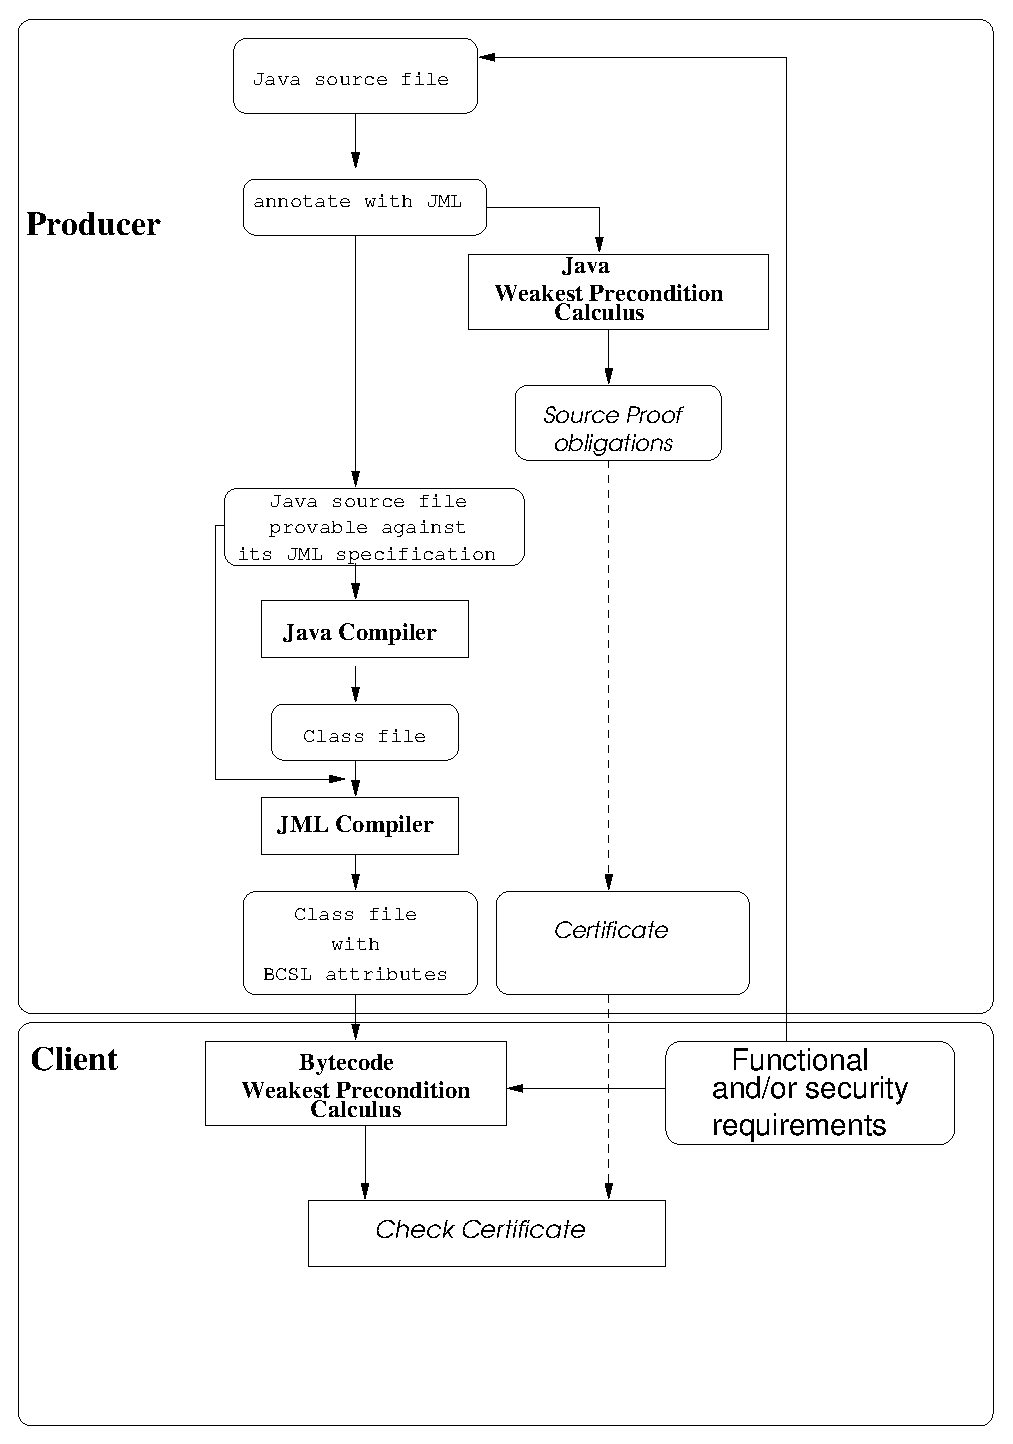
\epsfig{file=architecture.eps, width=\linewidth}
\caption{The overall architecture for annotating and verifying code}
\label{architecture}
\end{center}
\end{figure}
%\clearpage

It describes a process that allows a client to trust a code produced by an untrusted code producer.

In the first stage of the process the client provides the functional and (or) security requirements to the producer. The requirements can be in different form:
\begin{itemize}
\item A specified interface that describes the application to be developed. In that case, the client has fully specified in JML the features that have to be implemented by the code producer.
\item An API with some restricted access to some method. In this case, the client can protect its system by restricting its usage (for example, if the client API provides transaction management facilities, a requirement can be for no nested transactions and the API method \texttt{open} for opening and method \texttt{close} for closing transactions can be annotated to ensure that \texttt{close} should not be called if there is no transaction running and \texttt{open} should not be called if there is already a running transaction).   
\end{itemize}

%OLD:
% In the development process, the producer uses Jack to check the client requirements and usually has to add JML annotations for this %In both cases, the code producer develops its application and proves that it fulfills the given requirements using Jack; %in most cases, to complete this task, some annotations have to be added to the code 
%e.g. loop invariants, class invariants, method preconditions and postconditions etc. In a standard, application only after specifying enough the source code, 
%have we got the annotated Java source files to feed to the JML compiler.

In the development process, the producer verifies if the client requirements are respected by generating verification conditions
over the source code and usually, he has to add JML annotations for this e.g. loop invariants, class invariants, method preconditions
 and postconditions etc. Usually, only after specifying enough the source code, 
have we got the annotated Java source files to feed to the JML compiler.



When the annotations are sufficient to prove the code, 
the Java file is then normally compiled with a Java compiler to obtain a 
class file. This class file is then extended with user defined attributes that contain the BCSL specification, resulting from the compilation of the JML specification. 
At this stage, the Java class files contain all the information that will allow the client to check it. 
 %OLD
%In particular, the client will generate proof obligations from the untrusted annotated bytecode and his security requirements 
%(expressed in a suitable form) as shown in figure~\ref{architecture}. Proof obligations are formulas which, if provable, guarantee the bytecode correctness.
%The latter are then proved , for instance, with JACK (see section \ref{prelim}). If the client succeeds in proving 
%the verification conditions, he can trust the unknown code. Currently the framework does not support sending both the proof and the 
%bytecode to the client, which is the next step in our work.
In particular, the client will generate proof obligations from the untrusted annotated bytecode and his security requirements 
(expressed in a suitable form) as shown in figure~\ref{architecture}. Proof obligations are formulas which, if provable, guarantee the bytecode correctness.
The latter are then proved with a theorem prover (possibly interactively). If the client succeeds in proving 
the verification conditions, he can trust the unknown code. Currently the framework does not support sending both the proof and the 
bytecode to the client, which is the next step in our work.

%OLD
%To implement this architecture, we have defined a compiler from JML to BCSL; the JML compilation results in an extension of the class file format; 
%we have implemented a tool to insert those special attributes in the class file and we have extended the JACK framework to generate proof obligations at bytecode 
%level and to prove them with the plugged JACK provers (as explained in the introduction). 
%The coming sections introduce those features.  

To implement this architecture we use JACK as a verification condition generator both on the consumer and the
producer side. JACK is a plugin for the eclipse\footnote{http://www.eclipse.org} integrated development environment for Java. Originally, the tool was designed as verification condition generator for Java source programs against their JML specification. JACK can interface with several theorem provers (AtelierB, Simplify, Coq, PVS). We have extended the tool with a compiler from JML to BCSL and a bytecode verification condition generator. In the following we introduce the BCSL language, the JML compiler and the bytecode weakest precondition calculus which underlines the bytecode verification condition generator.
 
%the JML compilation results in an extension of the class file format; we have implemented a tool to insert those special attributes in the class file and we have extended 
%the JACK framework to generate proof obligations at bytecode level and to prove them with the plugged JACK provers (as explained in the introduction). 
%The coming sections introduce those features.  


\section{JACK's User Interface}\label{SecUI}

One of the features that distinguish JACK from other program
verification tools is the integration in the IDE Eclipse. This ensures
a seamless integration of formal methods in the application
development process: the application developer does not have to learn
the peculiarities of a new tool, and does not have to switch tools to
apply formal verification techniques.

The integration in Eclipse consists of two parts: an extension of the
standard Java perspective with special JACK-related actions (checking a
specification, calling an automatic prover \emph{etc.}), and a
special JACK perspective to inspect the generated proof
obligations.

\subsection{Extension of the Java Perspective in Eclipse}

The standard Java perspective of Eclipse is extended with several
JACK-specific features. Menus are added to set the defaults for the
different specification constructs. Further, there are buttons and
menu-options to ``compile'' a JML specification, (\emph{i.e.}\ type
check and generate proof obligations), call an automatic prover on all
the generated proof obligations (either Simplify or a special
Coq tactic), or change to the special JACK perspective.  

Checking the JML specification is not done automatically, while
editing the file (as is done for Java); instead the user has to launch
this action explicitly. At the time this interface was developed,
adding such automatic checks required too many changes to the
internals of Eclipse, which were not default available. However, in
the mean time such a feature has been developed within the JMLEclipse
project\footnote{See
\texttt{http://jmleclipse.projects.cis.ksu.edu/}.}. This project also
provides syntax highlighting of JML specifications in Eclipse's Java
perspective. All this could be integrated with the JACK interface. 

%It is future work to integrate this with the JACK interface.
%%(\emph{e.g.}\ the JMLEclipse project does not accept the keywords that
%JACK adds to JML. 

Finally, another important constraint is the interface's
responsiveness. An IDE is supposed to be used interactively, and the
developer should never have to wait long for a result. Proof
obligation generation is no problem for this, but calling an automatic
prover on the generated proof obligations can take a significant
amount of time. Therefore, the prover is called in a non-blocking way,
launching a special window that allows to see the progress of the
task.

\subsection{A Proof Obligation Inspection Perspective}

An important feature of JACK is that one can inspect the different
generated proof obligations. Moreover, one does not have to understand
the specific specification language of the prover that is being used;
instead the proof obligations can be viewed in a Java/JML-like syntax
(but of course, one can also choose to see the proof obligations as
they are generated for a specific theorem prover).

\begin{figure}[t!]
%julien: at my desk it makes things bugs....
% \epsfig{file=screen1.ps,angle=270,width=\textwidth}
% the following work better (for me, with the makefile)
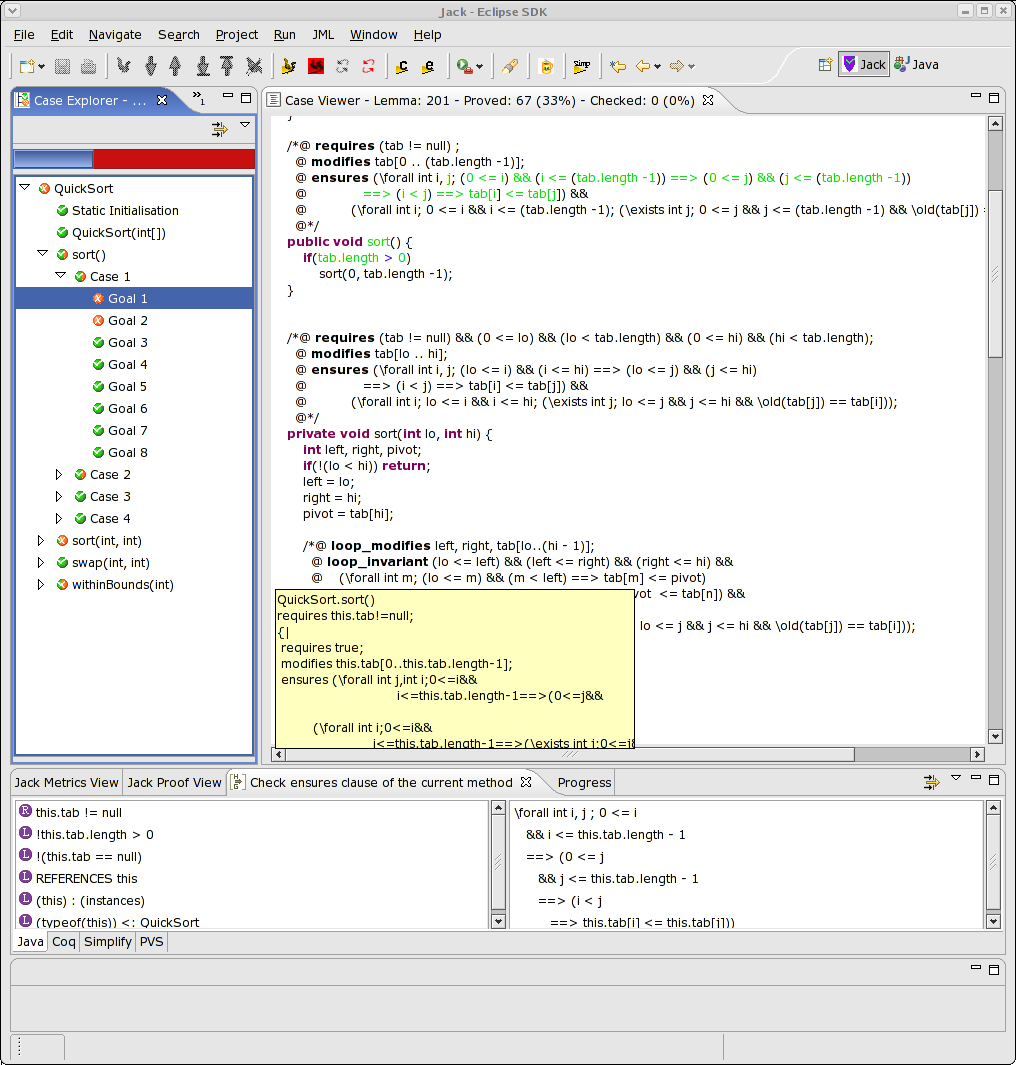
\epsfig{file=screen1, width=\textwidth}
\caption{JACK's proof obligation inspection perspective}\label{FigJackPerspective}
\end{figure}

%\begin{figure}[th!]
%    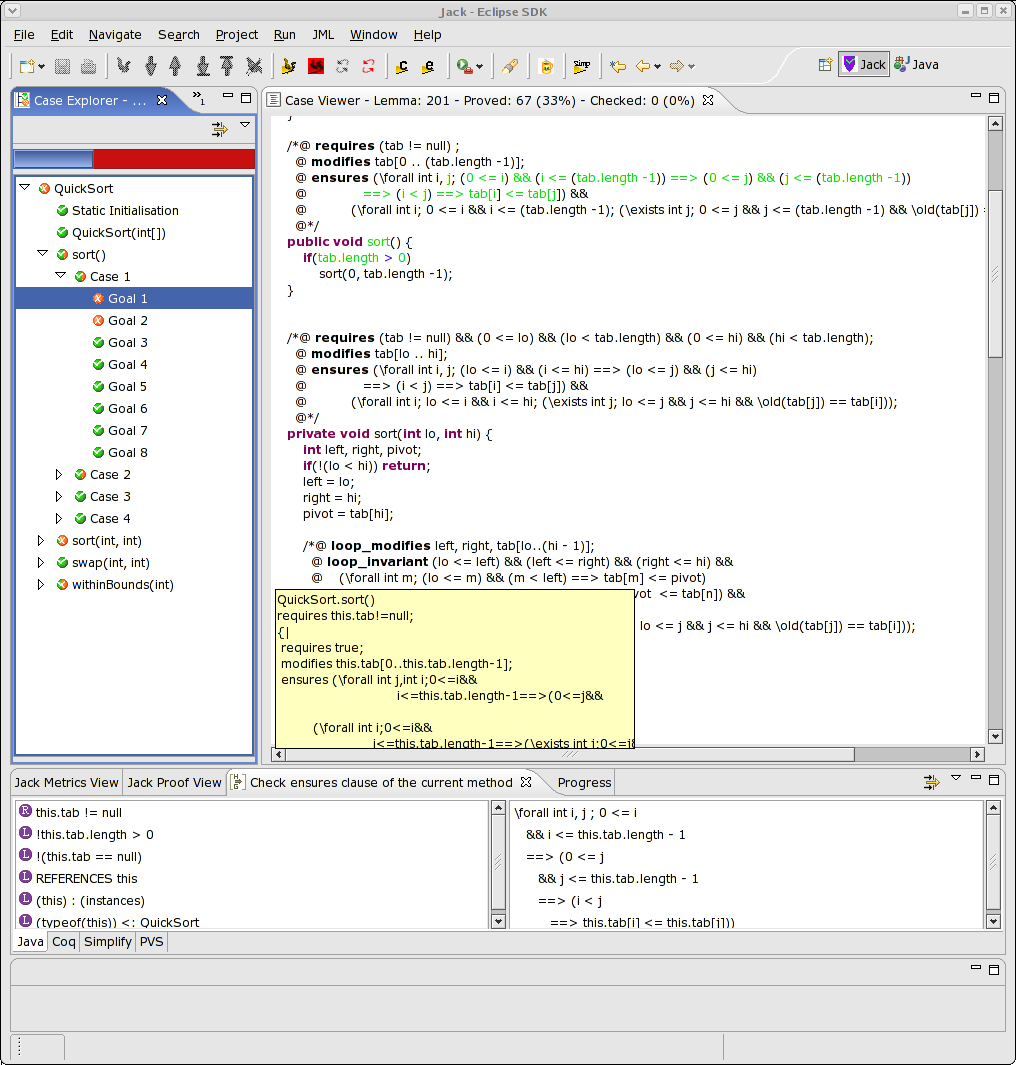
\includegraphics[width=\textwidth]{screen1}
%\caption{JACK's proof obligation inspection perspective}\label{FigJackPerspective}
%\end{figure}
%JACK's proof obligation inspection perspective provides the following information:
%\begin{itemize}
%\item information concerning the current proof status;
%\item the class methods with their lemmas;
%\item the source code; and
%\item the currently selected proof obligation (goal and hypotheses).
%\end{itemize}

Figure~\ref{FigJackPerspective} shows the inspection of a proof obligation
for the method \texttt{sort} in the QuickSort example of
Figure~\ref{FigJMLSpec}. The left upper windows allows one to browse
the proof obligations for the current class. Proven obligations are
ticked, the others are marked with a cross. The right window shows the
original source code, where the path through the code that corresponds
to the current proof obligation is coloured, together with the
relevant part of the method specification. Different colours are used
to indicate different cases, \emph{i.e.}\ to distinguish normal from
exceptional execution, and to mark that extra information is
available, such as a method specification, or the result of a
conditional expression.  The bottom window shows the proof obligation:
the left half contains the hypotheses, marked with letters indicating
their origin, \emph{e.g.}\ a hypothesis marked R originates from the
method's requires clause, while a hypothesis marked L is derived from
local declarations within the method. The right half of the window
shows the actual goal that has to be proven. The window name
highlights once again that this proof obligation originates from the
postcondition. Finally, notice that the proof obligation is here
displayed in Java syntax, but that buttons are available to change to
Coq, Simplify or PVS syntax.

%\marginpar{MH: Say something about 'manual check' option for proof
%obligations}

The user can use the proof obligation inspection view to inspect the
different (unproven) proof obligations, and to launch different
(interactive or specialised) provers to prove the remaining proof
obligations.



\section{Generating JML Annotations}\label{SecAnnotGen}

While JML is easily accessible to Java developers, actually writing
the specifications of an application is labour-intensive and
error-prone, as it is easy to forget some annotations. There exist
tools which assist in writing these annotations,
\emph{e.g.}, Daikon~\cite{ErnstCGN01} and Houdini~\cite{FlanaganL01}
use heuristic methods to produce annotations for simple safety and
functional invariants.  However, these tools cannot be guided by the
user---they do not require any user input---and in particular cannot
be used to generate annotations from realistic security policies.

Within JACK, we have implemented several algorithms to generate
annotations. We can distinguish two goals for annotation
generation. The first is to reduce the burden of annotation writing by
generating as much ``obvious'' annotations as possible. Given an
existing, unannotated, application, one first generates these obvious
annotations automatically, before developing the more interesting
parts of the specification. The second goal is to encode high-level
properties by encoding these with simple JML annotations, that are
inserted at all appropriate points in the application, so that they
can be checked statically.  JACK implements algorithms for both goals,
as described in this section.


\subsection{Generation of Preconditions}

%The first algorithm is a simple static analysis on the
%program text, which generates frame conditions. Whenever it sees
%assignments or method calls that change (specification) public fields,
%these fields are added to the method's assignable clause. The
%algorithm uses a safe over-approximation: whenever it encounters
%references that might be aliased, it generates a clause
%\texttt{assignable \bsl everything;}.

%JACK implements two different algorithms to generate ``obvious''
%annotations. 
JACK implements an algorithm to generate ``obvious'' minimal
preconditions to avoid null-pointer and array-out-of-bounds
exceptions. This algorithm re-uses the implementation of the
wp-calculus: it computes the weakest precondition for the
specification
\texttt{signals (NullPointerException) false;} (resp. \texttt{signals
(ArrayIndexOutOfBoundsException) false;}) and inserts this as 
annotations in the code.

%\marginpar{MH: Example with more useful assignable clause?}

\begin{figure}[t!]
{\small
\begin{verbatim}
/*@ requires this.tab!=null;
    signals (Exception) false;
  @*/
public void sort() {if(tab.length > 0) sort(0, tab.length -1);}

/*@ requires this.tab!=null && 0<=j && j<this.tab.length &&
             0<=i && i<this.tab.length;
    signals (Exception) false;
 @*/
public void swap(int i, int j) {int tmp; tmp = tab[i]; 
                                tab[i] = tab[j]; tab[j] = tmp;}
\end{verbatim}
}
\caption{Obvious annotations generated for a fragment of class
\texttt{QuickSort}}\label{FigAnnotSpec} 
\end{figure}

As an example, Figure~\ref{FigAnnotSpec} shows the annotations that
are generated for some methods of the class \texttt{QuickSort} of
Figure~\ref{FigJMLSpec}.  It is important to realise that the
specifications that are generated might not be very spectacular, but
that they are generated \emph{automatically}. % can help significantly to
% reduce the
%burden of annotation writing.

The annotation generation can be further improved by applying a simple
analysis on the generated annotations. Often it is the case that the
preconditions that are generated for the fields of the class are the
same for (almost) all methods. In that case, this condition is likely
to be a class invariant, and instead of generating a precondition for
each method, it would be more appropriate to generate a single class
invariant. For example, for the class
\texttt{QuickSort}, this would produce an annotation
\texttt{invariant this.tab!=null;}. %It is future work to implement
%this.

\subsection{Encoding of Security Policies}

Another difficulty when writing annotations is that a conceptually
simple high-level property can give rise to many different
annotations, scattered through the code, to encode this property. This
is typically the case for many security policies. Current software
practice for the development of applications for trusted personal
devices is that security policies give rise to a set of \emph{security
rules} that should be obeyed by the implementation. Obedience to these
rules is established by manual code inspection; however it is
desirable to have tool support for this, because a typical security
property may involve several methods from different classes.  Many of
the security rules can be formalised as simple automata, which are
amenable to formal verification. Therefore, we propose a method that
given a security rule, automatically annotates an application, in such
a way that if the application respects the annotations then it also
respects the security policy. Thus, it is not necessary for the user
to understand the generated annotations, he just has to understand 
the security rules.

The generation of annotations proceeds in two phases: first we
generate core-annotations that specify the behaviour of the methods
directly involved, and next we propagate these annotations to all
methods directly or indirectly invoking the methods that form the core
of the security policy. The second phase is necessary because we are
interested in static verification. The annotations that we generate
all use only JML static ghost variables; therefore the properties are
independent of the particular class instances available. 

As a typical example of the kind of security rules our approach can
handle, we consider the atomicity mechanism in Java Card (Java for
smart cards) (\cite{PavlovaBBHL04} gives more examples of such
security rules). A smart card does not include a power supply, thus a
brutal retrieval from the terminal could interrupt a computation and
bring the system in an incoherent state. To avoid this, the Java Card
specification prescribes the use of a transaction mechanism to control
synchronised updates of sensitive data. A statement block surrounded
by the methods \texttt{beginTransaction()} and
\texttt{commitTransaction()} can be considered atomic.
If something happens while executing the transaction (or if
\texttt{abortTransaction()} is executed), the card will
roll back its internal state to the state before the transaction was
begun. To ensure the proper functioning and prevent abuse of this
mechanism, applications should respect for example the following
security rules. 

\begin{quote}
\textbf{No nested transactions} Only one level of transactions
is allowed.\smallskip\\
\textbf{No exception in transaction} All exceptions that may be thrown
inside a transaction, should also be caught inside the
transaction.\smallskip\\
\textbf{Bounded retries}
No pin verification may happen within a transaction.
\end{quote} 
The second rule ensures that a transaction will always be closed;
if the exception would not be caught, \texttt{commitTransaction}
would not be executed. The last rule avoids the possibility to abort
the transaction every time a wrong pin code has been entered. As this
would roll back the internal state to the state before the transaction
was started, this would also reset the retry counter, thus allowing an
unbounded number of retries. Even though the specification of the Java
Card API prescribes that the retry counter for pin verification cannot
be rolled back, in general one has to check this kind of properties.

Such properties can be easily encoded with automata, describing in
which states a certain method is allowed to be called. Based on this
automata, we then generate core-annotations. For example, the
atomicity properties above give rise to core-annotations for the
methods related to the transaction mechanism declared in class
\texttt{JCSystem} of the Java Card API. A static ghost variable 
\begin{verbatim}
/*@ static ghost int TRANS == 0; @*/
\end{verbatim}
is declared, that is used to keep track of whether there is a
transaction in progress.  To specify the \textbf{No nested
transactions} property, the core-annotations for method
\texttt{beginTransaction} are the following. 

\begin{verbatim}
/*@ requires TRANS == 0;
  @ assignable TRANS;
  @ ensures TRANS == 1; @*/
public static native void beginTransaction() 
                          throws TransactionException;
\end{verbatim}
Similar annotations are generated for \texttt{commitTransaction} and
\texttt{abort\-Trans\-action} (\cite{PavlovaBBHL04} also
describes the generated core-annotations for the other
properties). After propagation, these annotations are sufficient to
check for the absence of nested transaction.  To understand why
propagation is necessary, suppose we are checking the \textbf{No
nested transactions} property for an application, containing the
following fragment (where
\texttt{m} does not call any other methods, and does not contain any
set annotations).

\begin{verbatim}
void m() { ... // some internal computations
           JCSystem.beginTransaction();
           ... // computations within transaction
           JCSystem.commitTransaction(); }
\end{verbatim}

When applying static verification on this code fragment, the
core-annotations for \texttt{beginTransaction} will give rise to a
proof obligation that the precondition of method
\texttt{m} implies that there is no transaction in progress,
\emph{i.e.}, \texttt{TRANS == 0} (since \texttt{TRANS} is not modified
by the code that precedes the call to \texttt{beginTransaction}). The
only way this proof obligation can be established is if the
precondition of \texttt{beginTransaction} is propagated as a
precondition for method \texttt{m}. In contrast, the precondition for
\texttt{commitTransaction} (\texttt{TRANS == 1}) does not have to be
propagated to the specification of \texttt{m}; instead it has to be
established by the postcondition of \texttt{begin\-Transaction},
because the variable \texttt{TRANS} is modified by this method.

In a similar way, the postcondition for the method
\texttt{commitTransaction} is propagated to the postcondition of
method \texttt{m}. This information can then be used for the
verification of yet another method, that contains a call to method
\texttt{m}. 

The propagation method not only propagates preconditions and normal
and exceptional postconditions, it also propagates assignable
clauses. We have shown that the algorithm that we use corresponds to
an abstract version of the wp-calculus (where we only consider
static variables). We have exploited this correspondence in the
implementation, by re-using the wp-calculus infrastructure to
implement the propagation algorithm. For a more formal treatment of
the propagation algorithm, and the correspondence statement, we refer
to~\cite{PavlovaBBHL04}.

To illustrate the effectiveness of our approach, we tested our method
on several industrial smart card applications, including the so-called
Demoney case study, developed as a research prototype by Trusted
Logic\footnote{See {\tt http://www.trusted-logic.fr}.}, and the PACAP
case study\footnote{See {\tt
http://www.gemplus.com/smart/rd/publications}.}, % /case-study
developed by Gemplus. Both examples have been explicitly developed as
test cases for different formal techniques, illustrating the different
issues involved when writing smart card applications. We used the
core-annotations as presented above, and propagated these throughout
the applications.  For both applications we found that they contained
no nested transactions, and that they did not contain attempts to
verify pin codes within transactions. However, in the PACAP
application we found transactions containing uncaught exceptions. All
proof obligations generated \emph{w.r.t.}~these properties are trivial
and can be discharged immediately. However, to emphasise the
usefulness of having a tool for generating annotations: we encountered
cases where a single transaction gave rise to twenty-three annotations
in five different classes. When writing these annotations manually, it
is all too easy to forget some.





The only semantics that are properly defined for AspectJ are defined
on Java bytecode \cite{weaving06,weaving04}. Therefore the only way to
implement a verification which is correct against the semantic of
AspectJ is by defining it on the bytecode level.  The program as well
as the annotations have to be compiled to Java bytecode and
and bytecode annotations. 

\subsubsection{Compilation of source code}
The source code of the Java program can be compiled with {\tt javac}.
The source code of {\tt before} and {\tt after}
advices does not have to be changed to be compiled to Java bytecode.
The advice just have to be named with a unique method name.
The around advices are more complex to compile as they contain the instruction
{\tt proceed()}. The proceed instruction is translated on bytecode as
a method that does not need to have a body, and which is specific 
to a single around advice that is compiled.


\subsubsection{Compilation of specifications} 
We have chosen the Bytecode Modelling Language (BML) to annotate the
bytecode. BML is a version of JML for bytecode, and there exists a
simple transformation from fully desugared JML to BML as presented
M. Pavlova PhD. thesis~\cite{PavlovaPhd}. Since our specifications
have been turned into simple JML (in Subsection~\ref{desugar}), we can
translate all the JML annotations to BML's. The advices all keep their
Pipa/JML specification unchanged except for the {\tt around} advice.
The {\tt ensures}, {\tt proceeds} and {\tt requires} that are the
nearer to the {\tt then} construct are removed from the {\tt around}
advice specifications. The {\tt proceed()} specific method takes its
specification from the one that were removed from the {\tt around} advice.
The {\tt requires} of the {\tt proceed()} equals the removed {\tt ensures}
and the ensures clause of the proceed() is the {\tt proceed} clause 
implies the {\tt requires} clause that were removed.
The frame condition should be easily inferred from the advice's 
static joint point.





\section{Support for Interactive Verification}\label{SecInteractive}
One of the interesting feature in Jack is its use for interactive 
verification. When automatic provers fail to solve a proof obligation,
the user can try to solve it interactivly (instead of the usual 
informal verification). It is comparable to what is done within the tool
 Krakatoa but Jack has the advantage to be integrated in Eclipse.
More specifically, Jack's case viewer allows to edit every proof that 
failed automatic verification separately and 
it also shows the proof source from the Java code. 
\subsection{The Coq plugin}
The generated  proof obligations are translated into Coq language, mostly
straight-forwardly. The main concern in this plugin is the proof readability,
and proof reusability.
That's why we developped a set of facilities for variable name handling,
pretty printing, the reuse of proofs, the ease to build the proofs and the 
user extensions.

\paragraph{Pretty printing}
In Jack, facilities for better readability already exists.
A difference is made between short variable names, 
when no other variable is named this way,
 and long variable names, when there can be an ambiguity. 
When doing interactive verification the scope of these disambiguations 
can be mistaken as Jack do it execution case wise and not lemma wise.
This disambiguation is redone (lemma wise) 
in the Coq plugin to add better proof readability.
The main pretty printing is done directly through Coq's own features for
 printing. Each proof obligation is passed to Coq top-level and the result of 
Coq's parsing is the proof obligation given to the user to view.

\paragraph{Lemma generation} 
A special attention has also be given when generating the proof obligations 
into a file. First it has a name composed of the full class name, the method
name, the execution case and the goal. It is done so the user can retrieve 
the proof obligation with Jack whenever he wants it. Each file is stocked
locally in a directory named {\tt proofs} 
for when the lemma is regenerated or reopened; the proof it was containing
can be replayed (and eventually fail if the conditions have changed too much).
The normal hypothesis are separated from the invariants; given different names.
It is specifically useful when a goal has been modified (and considered 
unproved) by the modification of an invariant. If the proof was not involving
the use of any invariant; it can be replayed without any changing.

\paragraph{Automations}
The interaction with the theorem has been made tighter than the usual 
interactive verification's one.
Jack has 3 {\it interactive-automatic} modes. 
By {\it automatic} we mean we 
try to apply a generic proof script to several goals, 
and if it fails we try another one. 
The three automatic modes are: the light mode, where we use a proof script
called lightAutoJack to prove the goals; 
the tough mode, where we use the proof script toughAutoJack, 
and the semi-auto mode where the user can write a proof script that will
be tried on several lemmas.



\subsection{Jack with Coq in Eclipse}
Jack's Coq plugin relies on a translation of Jack's Java logic in
Coq as well as several user extensions. Since everything is generated
inside the Eclipse's workspace, and the user extensions have to be 
developped as part of the interactive verification process,
 a smoother interaction of Coq within
the Eclipse environment was necessary.

\paragraph{Coq editor}
We added a way to interact directly with Coq through Eclipse's Java 
environment. It is a way to directly use Coq and edit Coq files within
Eclipse. It is alike what has been done for Isabelle in Proof General Eclipse 
\cite{WintersteinAL05}, but for Coq and in a more light-weight fashion.
It has keyboard shortcuts similar to CoqIde (the current Coq graphical
interface which is written in OCaml). 
The main feature we have is the outline view; 
which sums up the view of a Coq file in a tree-like fashion (especially useful
with to see modules hierarchy). There is a search by tags feature which
permits to search a whole project for the definition of a specific keyword; and
it is done incrementaly with Eclipse's builder feature. Of course, there is 
syntax highlighting for Coq files and you can interactively play a Coq file
as in the usual interactive provers IDE.


\paragraph{User extensions; tactics}

One of the key point in interactive verification is the level of difficulty
to manipulate the proof assistant in order to solve a proof obligation.
In order to help the user build proof scripts that are both intuitive
to read and to make, we have used the tactic mechanism of Coq.
These tactics are written in a pseudo language named Ltac \cite{DEL-00-LTAC}
which permits to combine primitive tactics.
The Coq plugin contains a library of those which, based on Jack's Coq 
implemented Java logic, can help for obvious or really specific proof steps
in Jack's proof obligations. All these tactics are situated in a library 
used when a new proof obligation is loaded. Tactics can also be used in 
really specific user oriented context. There is a special file called 
'user extension' which is meant to contain user-defined
special lemmas and special tactics.



\subsection{Towards native specifications}
\begin{figure}[t!]
{\small In JML we define:
\begin{verbatim}
/*@ public native class IntList {
     public native IntList cons (int i);
     public native static IntList create();
     ...
     public native static IntList toList (int [] tab);
   } @*/ \end{verbatim}}

{\small And in Coq:
\begin{verbatim}
Definition IntList := list t_int.
Definition IntList_create : IntList := nil .  
Definition IntList_cons:  t_int -> list t_int ->list t_int := 
            fun (i: t_int) (this: list t_int)  => (i :: this).
... \end{verbatim}}
\caption{The definition of native type \texttt{IntList}}\label{CoqAnnot} 
\end{figure}
User-extensions through the use of tactics are useful;
but sometimes users would like more expressivity: instead of having
tactics and extensions based solely on Jack's Java logic, a user could
build his own logic and use it with JML annotations. He could 
even use pre-existing logics and use them with his annotations. That is 
exactly the purpose of the native construct.


The native construct can be used to express some notions contained within
the annotation directly in the logic of the prover. If we define a native type 
IntList and we bind it to Coq list of integer type (Fig. \ref{CoqAnnot}), 
we can use the list library of Coq to do our proofs. The annotation of the
{\tt sort} method can be defined as annotations for our new type 
(Fig. \ref{sortnat}). We get more readable annotations;
the annotations are more natural for a Coq user because of relying upon Java
logic over the array, we get it defined with a Coq library.
The user can also define more easily lemmas to help prove some of the proof
obligations and to add automations for proof scripts.


\begin{figure}[t!]
{\small In JML we define:
\begin{verbatim}
//@ ghost IntList list;
/*@ requires (tab!=null) && list.equals(IntList.toList(tab))
    assignable tab[0 .. (tab.length -1)], list;
    ensures list.equals(IntList.toList(tab)) &&
             list.isSorted() && list.isPermutation();
 @*/
public void sort() {if(tab.length > 0) sort(0, tab.length -1);}\end{verbatim}}
\caption{\texttt{Sort} with natives}\label{sortnat} 
\end{figure}





\section{Conclusion and Future Work}\label{conclusion}
This article describes a bytecode weakest precondition calculus applied to a bytecode specification language (BCSL).
BCSL is defined as suitable extensions of the Java class file format.
Implementations for a proof obligation generator and a JML compiler to BCSL have been developed and are part of the Jack 1.8 release\footnote{http://www-sop.inria.fr/everest/soft/Jack/jack.html}.
At this step, we have built a framework for Java program verification.
 This validation can be done at source or at bytecode level in a common environment: for instance, to prove lemmas ensuring bytecode correctness all the current and future provers plugged in Jack can be used.

We are now aiming to complete our architecture for establishing trust in untrusted code - in particular extending the present work to a PCC architecture for establishing non trivial requirements.  
%Properties that can be verified are properties expressible in the JML specification language. Design by contract properties (used in interface design) can be easily expressed and sent through a network with this framework. What should be pointed out is that we do not deal with such low level properties like for example memory allocation or time constraints.What the approach proposes is suitable for verifying static properties (invariant) concerning objects: it can be relations between values, or conditions over expressions that the program treats.
In this way, several important directions for future work are:
\begin{itemize}
\item perform case studies and strengthen the tool with more experiments.
\item find an efficient representation and validation of proofs in order to construct a PCC framework for Java bytecode. We would like to build a PCC framework where the proofs are done interactively over the source code
and then compiled down to bytecode. Actually, as we stated in Section \ref{results} the proof obligations generated over a source program and over its compilation with non optimizing compiler are syntactically equivalent modulo name and types. 
\item an extension of the framework applying previous research results in automated annotation generation for Java bytecode (see~\cite{PBBHL}). The client thus will have the possibility to verify a security policy by propagating properties in the loaded code and then by verifying that the code verify the propagated properties.
%\item correctness of the semantics of the weakest precondition calculus proposed, which we will do over the bytecode operational semantics. 

\end{itemize}
%Finally, we are currently proving the correctness of the semantics of the weakest precondition calculus proposed, the proof is built over the bytecode operational semantics and will ensure the soundness of our weakest precondition calculus.



\bibliographystyle{plain}
\bibliography{bibli,fmco,../specification,/user/mhuisman/home/Research/Everest/Biblio/everest,/user/mhuisman/home/Research/Everest/Biblio/crossrefs}

\end{document}

